\documentclass{beamer}
\usepackage{tikz-cd}
\usepackage{dsfont}
\usepackage{comment}
\usepackage{mathabx,epsfig}
\usepackage{tcolorbox}

\newtheorem{conjecture}{Conjecture}
\newtheorem{conjeorem}{Conjeorem}

%\def\acts{\mathrel{\reflectbox{$\righttoleftarrow$}}}

\newcommand*\circled[1]{\tikz[baseline=(char.base)]{        \node[shape=circle,draw,inner sep=0.8pt] (char) {#1};}}

\mode<presentation>
{
  \usetheme{Boadilla}
  % or ...

  \setbeamercovered{invisible}
  % or whatever (possibly just delete it)
}

\setbeamertemplate{navigation symbols}{}
\setbeamertemplate{page number in head/foot}{}


\usepackage[english]{babel}
% or whatever

\usepackage[latin1]{inputenc}
% or whatever

\usepackage{times}
\usepackage[T1]{fontenc}
% Or whatever. Note that the encoding and the font should match. If T1
% does not look nice, try deleting the line with the fontenc.


\title[] % (optional, use only with long paper titles)
{Tight and non-Fillable Contact Structures on the Sphere}

\subtitle
{}

\author[Josua Kugler] % (optional, use only with lots of authors)
{Josua Kugler \texorpdfstring{\\}{,}results by Bowden\inst{\footnote{University of Regensburg}}, Gironella\inst{\footnote{University of Nantes}}, Moreno\inst{\footnote{Heidelberg University}}, Zhou\inst{\footnote{Morningside Center of Mathematics, CAS}}}

% - Give the names in the same order as the appear in the paper.
% - Use the \inst{?} command only if the authors have different
%   affiliation.

\institute% (optional, but mostly needed)
{Heidelberg University}
% - Use the \inst command only if there are several affiliations.
% - Keep it simple, no one is interested in your street address.

\date[MPI Leipzig] % (optional, should be abbreviation of conference name)
% - Either use conference name or its abbreviation.
% - Not really informative to the audience, more for people (including
%   yourself) who are reading the slides online

\subject{Symplectic and Contact Topology}
% This is only inserted into the PDF information catalog. Can be left
% out. 



% If you have a file called "university-logo-filename.xxx", where xxx
% is a graphic format that can be processed by latex or pdflatex,
% resp., then you can add a logo as follows:

% \pgfdeclareimage[height=0.5cm]{university-logo}{university-logo-filename}
% \logo{\pgfuseimage{university-logo}}



% Delete this, if you do not want the table of contents to pop up at
% the beginning of each subsection:
%\AtBeginSubsection[]
%{
 % \begin{frame}<beamer>{Outline}
  %  \tableofcontents[currentsection,currentsubsection]
  %\end{frame}
%}


% If you wish to uncover everything in a step-wise fashion, uncomment
% the following command: 

%\beamerdefaultoverlayspecification{<+->}

\makeatletter
    \newenvironment{withoutheadline}{
        \setbeamertemplate{headline}[default]
        \def\beamer@entrycode{\vspace*{-\headheight}}
    }{}
\makeatother

\begin{document}

\begin{frame}
  \titlepage
\end{frame}


% Structuring a talk is a difficult task and the following structure
% may not be suitable. Here are some rules that apply for this
% solution: 

% - Exactly two or three sections (other than the summary).
% - At *most* three subsections per section.
% - Talk about 30s to 2min per frame. So there should be between about
%   15 and 30 frames, all told.

% - A conference audience is likely to know very little of what you
%   are going to talk about. So *simplify*!
% - In a 20min talk, getting the main ideas across is hard
%   enough. Leave out details, even if it means being less precise than
%   you think necessary.
% - If you omit details that are vital to the proof/implementation,
%   just say so once. Everybody will be happy with that.

%\begin{frame}{Contact geometry and Reeb dynamics}

%A contact manifold is $(M^{2n+1},\xi=\ker \alpha)$, where $\alpha\wedge d\alpha^n>0$, $\alpha$ the contact $1$-form.

%\begin{center}
%\mbox{The Reeb field is} $R_\alpha: \;d\alpha(R_\alpha,\cdot)=0,\; \alpha(R_\alpha)=1.$  
%\end{center}

%\pause

%\begin{conjecture}[Weinstein] Every Reeb dynamics admits at least one periodic orbit. 
%\end{conjecture}

%\pause

%\begin{exampleblock}{}
%\begin{center}
%Geometry $\longleftrightarrow$  Dynamics
%\end{center}
%\end{exampleblock}

%Proved by Taubes in dimension $3$, open in higher dimension.
    
%\end{frame}

\begin{frame}
\begin{tcolorbox}
\Huge \begin{center}
    \textbf{Background}
\end{center}
\end{tcolorbox}
\end{frame}

\begin{frame}{Contact topology}

\textbf{Contact topology:} The study of contact manifolds, up to isotopy.

\medskip

\pause

\textbf{Fillability:} \emph{fillable} contact mflds are boundaries of symplectic mflds.

\pause

\begin{exampleblock}{Fillability question}  Which contact manifolds are \textbf{fillable}?
\end{exampleblock}

\pause

Eliashberg, Borman--Eliashberg--Murphy:

\begin{tcolorbox}
\textbf{Dichotomy:} Rigidity vs.\ Flexibility. 
\begin{itemize}
    \item \textbf{tight} \emph{(rigid/geometric)};
    \item  \textbf{overtwisted} \emph{(flexible/topological)}. 
\end{itemize}
\end{tcolorbox} 

\pause

\begin{theorem}[Eliashberg--Gromov]
Fillable contact manifolds are tight.
\end{theorem}

Converse is false (Etnyre--Honda, Massot--Niederkrueger--Wendl).

\end{frame}

\begin{frame}{Existence and classification}

\emph{Topological} obstruction: \emph{almost} contact structure, i.e.\ reduction of structure group to $U(n)\times \mathds 1$.

\begin{theorem}[Lutz--Martinet (dim 3), Casals--Pancholi--Presas (dim 5), Borman--Eliashberg--Murphy (any dim)]

Almost contact manifolds are contact, where the contact structure is \emph{overtwisted}.

\end{theorem}

\pause

\begin{exampleblock}{Tight manifolds}
How can \textbf{tight} contact manifolds be understood?
\end{exampleblock}
    
\end{frame}

\begin{frame}{Contact structures on spheres}

\begin{exampleblock}{Standard contact structure}
The standard contact structure is $(S^{2n-1},\xi)=\partial(B^{2n},\omega_{std})$.
\end{exampleblock}

\pause

\begin{theorem}[Eliashberg, '91] 
    On $S^3$, it is the unique tight contact structure.
\end{theorem} 

In particular, no tight and non-fillable contact structures on $S^3$.

    %\item Eliashberg ('91): $n\geq 2$, $S^{2n+1}$ has non-standard fillable  structures.
    %\item Ustilovsky ('99): $n\geq 2$, $S^{4n+1}$, infinitely many structures.
    %\item Ding--Geiges ('04): every odd sphere has non-standard contact structures.
    
    
    %\medskip
    
    %Uebele ('16), Alves--Meiwes ('19, dynamical properties), Lazarev ('20, flexible fillings),...
    


\end{frame}

\begin{frame}{Tight and non-fillable structures in $\dim \geq 5$}

\begin{theorem}[Bowden--Gironella--Moreno--Zhou '22-'24]
    For every $n \geq 2$, the sphere $\mathbb S^{2n+1}$ admits a tight, non-fillable contact structure that is homotopically standard.
\end{theorem}

\pause
\vspace*{1cm}
By connected sum with such an ``exotic'' sphere, it can be concluded
\begin{theorem}[Bowden--Gironella--Moreno--Zhou '22-'24]
In $\dim \geq 7$, if $M$ admits a tight structure, it also admits a tight and non strongly-fillable structure, in the same almost contact class.
\pause

In $\dim=5$, the same holds, if the first Chern class vanishes.
\end{theorem}
\end{frame}

\begin{frame}
\begin{tcolorbox}
\Huge \begin{center}
    \textbf{Tight and non-fillable spheres}
\end{center}
\end{tcolorbox}
\end{frame}

\begin{frame}{Giroux correspondence}

\begin{tcolorbox}
\textbf{Giroux:} Contact structures are \emph{supported} by open books.
\end{tcolorbox} 

\begin{figure}
    \centering
    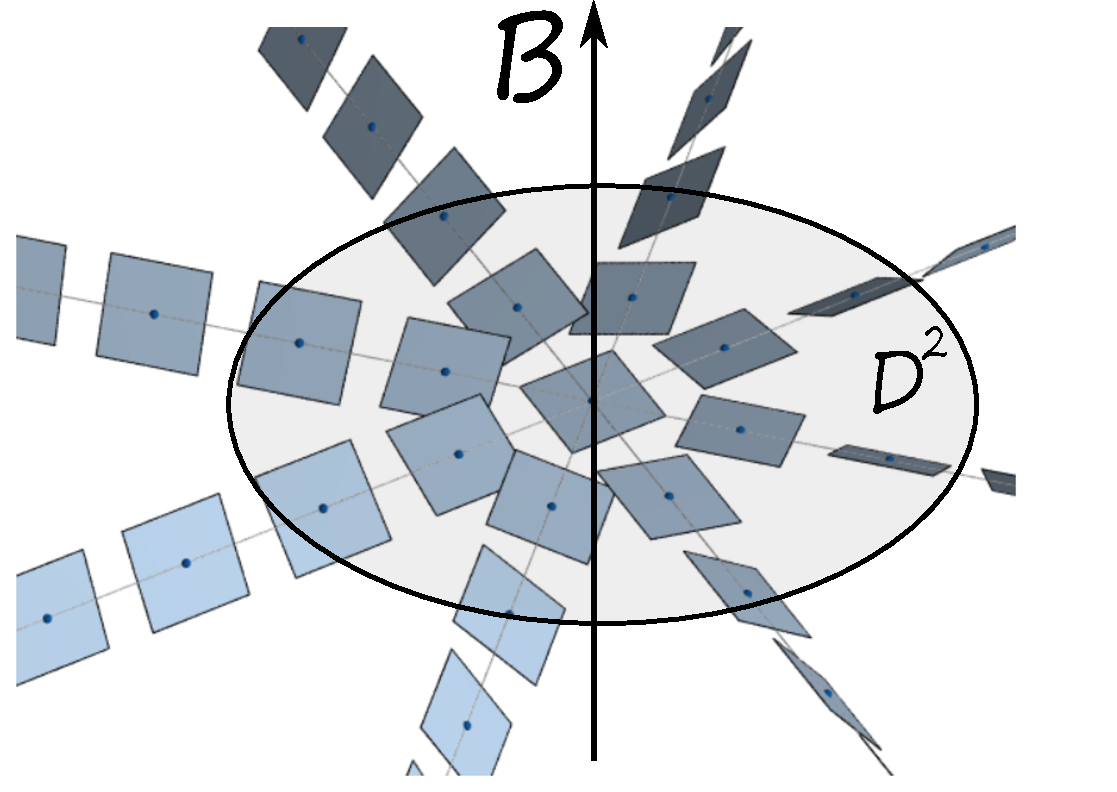
\includegraphics[width=0.6\linewidth]{standardctct.pdf}
    \caption{Supported contact structure.}
    \label{fig:adapted}
\end{figure}

\end{frame}

\begin{frame}{Bourgeois contact structures}
    \begin{theorem}[Bourgeois '02]
    Open book supporting $(M,\xi)\rightsquigarrow$ contact structure on $M\times \mathbb T^2$.
    \end{theorem}

 These are $\mathbb T^2$-equivariant.   
    
\end{frame}

\begin{frame}{Geometric construction}
    
    \textbf{Geometric construction:} Construct a tight and non-fillable contact structure on $\mathbb S^{2n+1}$:
    
    \medskip
    
    \pause

    \begin{itemize}
        \item Milnor open book on $\mathbb S^{2n-1}\overset{\text{Bourgeois}}{\rightsquigarrow}$ contact structure on $\mathbb S^{2n-1}\times \mathbb T^2$
    $\rightsquigarrow$ two $1$-surgeries = $\mathbb S^{2n-1}\times \mathbb S^2 \rightsquigarrow$ one $2$-surgery = $\mathbb S^{2n+1}.$

    \medskip

    \pause
    
    \item If $n\geq 3,$ surgeries are \emph{subcritical} $\rightsquigarrow$ by 'Eliashberg's' h-pple, Weinstein cobordism $\rightsquigarrow$ contact manifold $(\mathbb S^{2n+1},\xi_{ex})$.

    \end{itemize}

    \pause
    
    \medskip

    \begin{tcolorbox}
    \textbf{Claim:} $(\mathbb S^{2n+1},\xi_{ex})$ is tight and non-fillable.
    \end{tcolorbox}
    
\end{frame}

\begin{frame}{Tightness}

\textbf{Facts:} \begin{enumerate}
    \item Milnor open book $\Rightarrow$  algebraically tight Bourgeois manifold.
    \pause
    \begin{itemize}
        \item Algebraic tightness is vanishing of a certain contact homology algebra.
    \end{itemize}
    \pause
    \item Algebraic tightness is preserved under surgeries.
    \pause
    \item Algebraically tight $\implies$ tight.
\end{enumerate}

\pause

\vspace*{1cm}

\begin{tcolorbox}
    Milnor open book $\Rightarrow (\mathbb S^{2n+1},\xi_{ex})$ is \emph{tight}.
    \end{tcolorbox}

\end{frame}

\begin{frame}{Fillability}
    \begin{itemize}
        \item Pseudoholomorphic curves
        \item clever geometric construction
        \item homological obstruction
    \end{itemize}
\end{frame}

\begin{frame}
    \centering
    Thank you!
        
    \end{frame}

\begin{frame}{Fillability}

\textbf{Observation:} Bourgeois manifolds have convex decomposition 
$$\mathrm{OB}(\Sigma, \phi) \times \mathbb T^2=(\mathrm{OB}(\Sigma, \phi)\times \mathbb S^1)\times \mathbb S^1= V_+\times \mathbb S^1 \cup_\phi \overline{V}_-\times \mathbb S^1,$$ with $V_\pm=\Sigma \times D^*\mathbb S^1$, $\Sigma=$ page of the open book, $\phi=$ monodromy.

\pause

\begin{theorem}[Bowden--Gironella--Moreno]

$M=V\times \mathbb S^1=V_+\times \mathbb S^1\cup_\phi \overline{V_-}\times \mathbb S^1$ with convex decomposition, $N=\partial V_\pm$ dividing set. If $W$ is a symplectic filling of $M$, then
$$
H_*(N)\rightarrow H_*(V_\pm) \rightarrow H_*(W),
$$
induced by inclusion. Then second map is injective on image of the first.
\end{theorem}

Namely, if a homology class in $N$ survives in $V_\pm$, then it survives in the filling.
    
\end{frame}

\begin{comment}
\begin{frame}{Fillability}

\textbf{Fact:} 

\begin{enumerate}
    \item If $\dim \geq 7$, subcritical surgeries on $\mathbb S^{2n-1}\times \mathbb T^2$ can be pushed away from dividing set to $V_+$.
$$
\Rightarrow (\mathbb S^{2n+1},\xi_{ex}) \mbox{ still has a dividing set } N,
$$
with $H_n(N)\neq 0$.

\pause 
\item Homological obstruction theorem persists under surgery away from dividing set (capping cobordisms).
\end{enumerate}


\begin{figure}
    \centering
    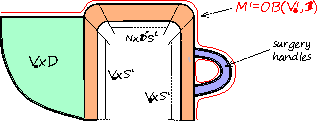
\includegraphics[width=0.68\linewidth]{blowdown_handle.pdf}
    \caption{Capping cobordism.}
    \label{fig:capping_cobordism}
\end{figure}

\end{frame}
\end{comment}

\begin{frame}

\textbf{Proof:} $W$ filling of $(\mathbb S^{2n+1},\xi_{ex})$:

$$
0\neq H_n(N) \xrightarrow{\text{nontrivial}} H_n(W).
$$
However, this factors as
$$
0\neq H_n(N) \rightarrow H_n(\partial W = \mathbb S^{2n+1})=0 \rightarrow H_n(W),
$$
contradiction.
\end{frame}

\end{document}